\section{Объявления типов и сопоставление с образцом}
\label{sec:types_and_pattern_matching}

С помощью типов определёных в Objective CAML мы можем определять структурные
типы, при помощи кортежей или списков. Но в некоторых случаях бывает необходимо
определить новые типы для описания специальных структур. В Objective CAML,
объявления типов рекурсивны и могут быть параметризованы переменными типа, как в
случае \texttt{'a list} который мы уже обсуждали. Вывод типов принимает во
внимание новые объявления для определения типов выражений. Конструкция значений
новых типов использует конструктор описанный определением типа. Особой
возможностью языков семейства ML является сопоставление с образцом, которое
обеспечивает простой метод доступа к компонентам (полям) структур данных.
Определение функции соответствует чаще всего сопоставлению с образцом по одному
из ее параметров, что позволяет определять функции для различных случаев.

Для начала, продемонстрируем механизм сопоставления на существующих типах и
затем опишем различные объявления структурных типов, конструкций таких
переменных и доступ к компонентам по сопоставлению с образцом.

\subsection{Сопоставление с образцом}

 Образец (по английски \texttt{pattern}) строго говоря не совсем выражение
Objective CAML. Речь скорее идёт о корректной компоновке (синтаксической и с
точки зрения типов) элементов, таких как константы базовых типов (\texttt{int,
bool, char $\ldots$}), переменные, конструкторы и символ \texttt{\_}, называемый
универсальным образцом. Другие символы служат для записи шаблона, которые мы
опишем по ходу.

Сопоставление с образцом применяется к значениям, оно служит для распознания
формы этих значений и позволяет определять порядок вычислений. С каждым образцом
связано выражение для вычисления.

Синтаксис:

\begin{lstlisting}[language=OCaml]
match expr with
| p1 -> expr1
:
| pn -> exprn
\end{lstlisting}

Выражение \texttt{expr} последовательно сопоставляется (фильтруется) с разными
образцами \texttt{p1, $\ldots$, pn}. Если один из образцов (например
\texttt{pi}) соответствует значению \texttt{expr}, то соответствующее
ответвление будет вычислено (\texttt{expri}). Образцы \texttt{pi} одинакового
типа, так же как и \texttt{expri}. Вертикальная черта перед первым образцом не
обязательна.

\subsubsection{Пример}

Приведём два способа, при помощи сопоставления с образцом, определения функции
\texttt{imply} типа \texttt{(bool * bool)->bool}, реализующую логическую
импликацию. Образец для пар --- \texttt{(,)}.

Первая версия перечисляет все возможности, как таблица истинности.

\begin{lstlisting}[language=OCaml]
# let imply v = match v with
     (true,true)   -> true
   | (true,false)  -> false
   | (false,true)  -> true
   | (false,false) -> true;;
val imply : bool * bool -> bool = <fun>
\end{lstlisting}

Используя переменные группирующие несколько случаев, мы получаем более
компактное определение.

\begin{lstlisting}[language=OCaml]
# let imply v = match v with
     (true,x)  -> x
   | (false,x) -> true;;
val imply : bool * bool -> bool = <fun>
\end{lstlisting}

Обе версии \texttt{imply} выполняют одну и ту же функцию, то есть они возвращают
одинаковые значения, для одинаковых входных аргументов.

\subsubsection{Линейный образец}

Образец обязательно должен быть линейным, то есть определённая переменная не
может быть использована дважды. Мы могли бы написать:

\begin{lstlisting}[language=OCaml]
# let equal c = match c with
      (x,x) -> true
    | (x,y) -> false;;
Error: Variable x is bound several times in this matching
\end{lstlisting}

Но для этого компилятор должен уметь реализовывать тесты на равенство, что
приводит к множеству проблем. Если мы ограничимся физическим значением
переменных, то мы получим слишком \enq{слабую} систему, не в состоянии,
например, распознать равенство между двумя списками \texttt{[1; 2]}. Если же мы
будет проверять на структурное равенство, то рискуем бесконечно проверять
циклические структуры. Рекурсивные функции, например, это циклические структуры,
но мы так же можем определить рекурсивные значения не являющиеся функциями
(см.\ref{??}).

\subsubsection{Универсальный образец}

Символ \texttt{\_} совпадает со всеми возможными значениями --- он называется
универсальным. Этот образец может быть использован для сопоставления сложных
типов. Воспользуемся им для определения ещё одной версии функции \texttt{imply}:

\begin{lstlisting}[language=OCaml]
# let imply v = match v with
         (true,false) -> false
       |   _          -> true;;
val imply : bool * bool -> bool = <fun>
\end{lstlisting}

Сопоставление должно обрабатывать все случаи, иначе компилятор выводит
сообщение:

\begin{lstlisting}[language=OCaml]
# let is_zero n = match n with  0 -> true ;;
Warning 8: this pattern-matching is not exhaustive.
Here is an example of a value that is not matched:
1
val is_zero : int -> bool = <fun>
\end{lstlisting}

В случае если аргумент не равен 0, функция не знает какое значение должно быть
возвращено. Для исправления добавим универсальный образец:

\begin{lstlisting}[language=OCaml]
# let is_zero n = match n with
    0 -> true
  | _ -> false ;;
val is_zero : int -> bool = <fun>
\end{lstlisting}

Если во время выполнения ни один образец не выбран, возбуждается исключение:

\begin{lstlisting}[language=OCaml]
# let f x = match x with 1 -> 3 ;;
Warning 8: this pattern-matching is not exhaustive.
Here is an example of a value that is not matched:
0
val f : int -> int = <fun>
# f 1 ;;
- : int = 3
# f 4 ;;
Exception: Match_failure ("", 77, -33).
\end{lstlisting}

Исключение \texttt{Match\_Failure} возбуждено при вызове \texttt{f 4} и если оно
не обработано, то вычисление останавливается (см. \ref{??}).

\subsubsection{Комбинация образцов}

Комбинация образцов позволяет получить новый образец, который может разложить
значение в соответствии с одним или другим из начальных шаблонов.

Синтаксис

$$
p_1 | \dots | p_n
$$

Эта форма создаёт новый образец из комбинации мотивов $p_1, \ldots, p_n$, с
единственным ограничением --- каждый из этих образцов должен содержать
константные значения либо универсальный образец.

Следующий пример показывает как проверить является ли входной символ гласной
буквой.

\begin{lstlisting}[language=OCaml]
# let is_a_vowel c = match c with
    'a' | 'e' | 'i' | 'o' | 'u' | 'y' -> true
  | _ -> false ;;
val is_a_vowel : char -> bool = <fun>
# is_a_vowel 'i' ;;
- : bool = true
# is_a_vowel 'j' ;;
- : bool = false
\end{lstlisting}

\subsubsection{Параметризованное сопоставление}

Параметризованное сопоставление используется в основном для определения функций
выбора. Для облегчения записи подобных определений, конструктор
\texttt{function} разрешает следующее сопоставление одного параметра.

Синтаксис

\begin{lstlisting}[language=OCaml]
function | p1 -> expr1
    | p2 -> expr2
    :
    | pn -> exprn
\end{lstlisting}

Вертикальная черта перед первым образцом не обязательна. Каждый раз при
определении функции, мы используем сопоставление с образцом. Действительно,
конструкция \texttt{function x -> expression} является определением
сопоставления по уникальному образцу одной переменной. Можно использовать эту
особенность в простых шаблонах:

\begin{lstlisting}[language=OCaml]
# let f = function (x,y) -> 2*x + 3*y + 4 ;;
val f : int * int -> int = <fun>
\end{lstlisting}

Форма

\begin{lstlisting}[language=OCaml]
 function p1 -> expr1 | ... | pn -> exprn 
\end{lstlisting}

эквивалентна

\begin{lstlisting}[language=OCaml]
function expr -> match expr with p1 -> expr1 | ... | pn -> exprn
\end{lstlisting}

Используя схожесть определения на (см. \ref{sec:def_func_val_let}), мы бы
написали:

\begin{lstlisting}[language=OCaml]
# let f (x,y) = 2*x + 3*y + 4 ;;
val f : int * int -> int = <fun>
\end{lstlisting}

Но подобная запись возможна лишь в случае если фильтруемое значение принадлежит
к типу с единственным конструктором, иначе сопоставление не является
исчерпывающим:

\begin{lstlisting}[language=OCaml]
# let is_zero 0 = true ;;
Warning 8: this pattern-matching is not exhaustive.
Here is an example of a value that is not matched:
1
val is_zero : int -> bool = <fun>
\end{lstlisting}

\subsubsection{Присвоение имени фильтруемому значению}

Иногда при сопоставлении с образцом, бывает необходимо дать имя всему образцу
или лишь его части. Следующая синтаксическая форма вводит ключевое слово as,
которое ассоциирует имя образцу.

Синтаксис

\begin{lstlisting}[language=OCaml]
(p as nom)
\end{lstlisting}

Это бывает полезно когда необходимо разбить значение на части, сохраняя при этом
его целостность. В следующем примере функция возвращает наименьшее рациональное
число из пары. Каждое рациональное число представлено числителем и знаменателем.

\begin{lstlisting}[language=OCaml]
# let min_rat pr = match pr with
   ((_,0),p2) ->  p2
 | (p1,(_,0)) ->  p1
 | (((n1,d1) as r1), ((n2,d2) as r2)) ->
         if (n1 *  d2 ) < (n2 * d1) then r1 else r2;;
val min_rat : (int * int) * (int * int) -> int * int = <fun>
\end{lstlisting}

Для сравнения двух рациональных чисел, необходимо разбить их для именования
числителя и знаменателя \texttt{(n1, n2, d1 и d2)}, но так же для собирания в
одно целое начальные пары (\texttt{r1} или \texttt{r2}). Конструкция позволяет
дать имена частям значения --- это избавляет от реконструкции рационального
числа при возвращении результата.

\subsubsection{Сопоставление с ограничением}

Сопоставление с ограничением соответствует вычислению условного выражения сразу
после сопоставления с образцом. Если это выражение возвращает значение
\texttt{true}, то выражение соответствующее этому образцу будет вычислено, иначе
сопоставление будет продолжаться дальше.

Синтаксис:

\begin{lstlisting}[language=OCaml]
match expr with
:
| pi when condi -> expri
:
\end{lstlisting}

В следующем примере используется два ограничения для проверки равенства двух
рациональных чисел.

\begin{lstlisting}[language=OCaml]
# let eq_rat cr = match cr with
   ((_,0),(_,0)) ->  true
 | ((_,0),_) ->  false
 | (_,(_,0)) ->  false
 | ((n1,1), (n2,1)) when n1 = n2 -> true
 | ((n1,d1), (n2,d2)) when ((n1 * d2) = (n2 * d1)) -> true
 | _ -> false;;
val eq_rat : (int * int) * (int * int) -> bool = <fun>
\end{lstlisting}

Если при фильтрации четвёртого образца ограничение не выполнится, то
сопоставление продолжится по пятому образцу.

{\it Предупреждение}

При проверке исчерпываемости сопоставления Objective CAML предполагает что
условное выражение может быть ложным. В следствии, верификатор не учитывает этот
образец, так как не возможно знать до выполнения сработает ограничение или нет.
Исчерпываемость следующего фильтра не может быть определена.

\begin{lstlisting}[language=OCaml]
# let f = function x when x = x  -> true;;
Warning 25: bad style, all clauses in this pattern-matching are guarded.
val f : 'a -> bool = <fun>
\end{lstlisting}

\subsubsection{Образец интервала символов}

При сопоставлении символов, неудобно описывать комбинацию всех образцов, которая
соответствует интервалу символов. Действительно, для того чтобы проверить
является ли символ буквой, необходимо написать как минимум 26 образцов и
скомбинировать их. Для символьного типа разрешается запись следующего шаблона:

Синтаксис

\begin{lstlisting}[language=OCaml]
'c1' .. 'cn'
\end{lstlisting}

что соответствует \texttt{'c1' | 'c2' | ...| 'cn'}

К примеру образец

\begin{lstlisting}[language=OCaml]
'0' .. '9'
\end{lstlisting}

соответствует образу

\begin{lstlisting}[language=OCaml]
'0' | '1' | '2' | '3' | '4' | '5' | '6' | '7' | '8' | '9'.
\end{lstlisting}

Первая форма быстрее и проще воспринимается при чтении.

{\it Предупреждение}

Это особенность является расширением языка и может измениться в следующих
версиях.

Используя комбинированные образцы и интервалы, напишем функцию по определению
символа по нескольким критериям.

\begin{lstlisting}[language=OCaml]
# let char_discriminate c = match c with
     'a' | 'e' | 'i' | 'o' | 'u' | 'y'
   | 'A' | 'E' | 'I' | 'O' | 'U' | 'Y'  -> "Vowel"
   | 'a'..'z' | 'A'..'Z' -> "Consonant"
   | '0'..'9' -> "Digit"
   |   _ -> "Other" ;;
val char_discriminate : char -> string = <fun>
\end{lstlisting}

Заметим, что порядок образцов важен, второе множество содержит первое, но оно
проверяется только после неудачи первого теста.

\subsubsection{Образцы списков}

Как мы уже видели список может быть:
\begin{itemize}
	\item либо пуст (в форме \texttt{[]})

	\item либо состоять из первого элемента (заголовок) и под–списка (хвост). В
этом случае он имеет форму \texttt{t::q}.
\end{itemize}

Обе эти записи могут быть использованы в образце при фильтрации списка.

\begin{lstlisting}[language=OCaml]
# let rec size x = match x with
     [] -> 0
   | _::tail_x -> 1 + (size tail_x) ;;
val size : 'a list -> int = <fun>
# size [];;
- : int = 0
# size [7;9;2;6];;
- : int = 4
\end{lstlisting}

Перепишем раннее показанный пример (см. \ref{sec:caml_kernel:examples})
используя сопоставление с образом для итерации списков.

\label{sec:caml_kernel:examples:lstlisting}

\begin{lstlisting}[language=OCaml]
let rec fold_left f a = function
    [] -> a
  | head::tail -> fold_left f (f a head) tail ;;
# fold_left (+) 0 [8;4;10];;
- : int = 22
\end{lstlisting}

\subsubsection{Объявление значения через сопоставлением с образцом}

Объявление значений само по себе использует сопоставление. \texttt{let x = 18}
сопоставляет образцы \texttt{x} со значением \texttt{18}. Любой образец
принимается как фильтр объявления, переменные образца ассоциируются со
значениями которые они сопоставляют.

\begin{lstlisting}[language=OCaml]
# let (a,b,c) = (1, true, 'A');;
val a : int = 1
val b : bool = true
val c : char = 'A'
# let (d,c) = 8, 3 in d + c;;
- : int = 11
\end{lstlisting}

Видимость переменных фильтра та же самая что у локальных переменных. Здесь
\texttt{c} ассоциировано с \texttt{'A'}.

\begin{lstlisting}[language=OCaml]
# a + (int_of_char c);;
- : int = 66
\end{lstlisting}

Как и любой фильтр, определение значения может быть не исчерпывающим.

\begin{lstlisting}[language=OCaml]
# let [x;y;z] = [1;2;3];;
Warning 8: this pattern-matching is not exhaustive.
Here is an example of a value that is not matched:
[]
val x : int = 1
val y : int = 2
val z : int = 3
# let [x;y;z] = [1;2;3;4];;
Warning 8: this pattern-matching is not exhaustive.
Here is an example of a value that is not matched:
[]
Exception: Match_failure ("", 98, -39).
\end{lstlisting}

Принимается любой образец, включая конструктор, универсальный и комбинированный.

\begin{lstlisting}[language=OCaml]
# let head :: 2 :: _ =  [1; 2; 3] ;;
Warning 8: this pattern-matching is not exhaustive.
Here is an example of a value that is not matched:
[]
val head : int = 1
# let _ = 3. +. 0.14 in "PI" ;;
- : string = "PI"
\end{lstlisting}

Последний пример мало интересен для функционального программирования, поскольку
значение 3.14 не именовано, и соответственно будет потерянно.

\subsection{Декларация типов}

Объявление типа --- это одна из других возможных фраз синтаксиса Objective CAML.
Она позволяет определить новые типы соответствующие обычным структурам данных
используемым в программах. Существует два больших семейства типов:
тип--произведение для кортежей или записей или тип--сумма для \texttt{union}.

Синтаксис:

\begin{lstlisting}[language=OCaml]
type nom = typedef ;;
\end{lstlisting}

В отличии от объявления переменных, объявление типов по умолчанию рекурсивно. То
есть объявления типов, когда они скомбинированы, могут объявлять взаимно
рекурсивные типы.

Синтаксис:

\begin{lstlisting}[language=OCaml]
type name1 = typedef1
and  name2 = typedef2
     :
and  namen = typedefn ;;
\end{lstlisting}

Объявления типов могут быть параметризованы переменной типа. Имя переменной типа
начинается всегда с апострофа (символ ').

Синтаксис

\begin{lstlisting}[language=OCaml]
type 'a nom = typedef ;;
\end{lstlisting}

В случае когда таких переменных несколько, параметры типа декларируются как
кортеж перед именем типа.

Синтаксис

\begin{lstlisting}[language=OCaml]
type ('a1 ...'an) nom = typedef ;;
\end{lstlisting}

Только те параметры, которые определены в левой части декларации, могут появится
в её правой части.


Замечание
Во время вывода на экран Objective CAML переименует параметры типа, первый в
\texttt{'a}, второй в \texttt{'b} и так далее. Мы всегда можем объявить новый
тип используя ранее объявленные типы.

Синтаксис:

\begin{lstlisting}[language=OCaml]
type name = type expression
\end{lstlisting}

Это полезно в том случае, когда мы хотим ограничить слишком общий тип:

\begin{lstlisting}[language=OCaml]
# type 'param paired_with_integer = int * 'param ;;
type 'a paired_with_integer = int * 'a
# type specific_pair = float paired_with_integer ;;
type specific_pair = float paired_with_integer
\end{lstlisting}

Без ограничения, выводится наиболее общий тип:

\begin{lstlisting}[language=OCaml]
# let x = (3, 3.14) ;;
val x : int * float = (3, 3.14)
\end{lstlisting}

Но мы можем использовать ограничитель типа для того, чтобы получить желаемое
имя:

\begin{lstlisting}[language=OCaml]
# let (x:specific_pair) = (3, 3.14) ;;
val x : specific_pair = (3, 3.14)
\end{lstlisting}

\subsection{Записи}

Запись --- это кортеж, в котором каждому полю присваивается имя на подобии
\texttt{record} в Pascal или \texttt{struct} в C. Запись всегда соответствует
объявлению нового типа. Для определения записи необходимо указать её имя, а так
же имя и тип для каждого поля записи.

Синтаксис:

\begin{lstlisting}[language=OCaml]
type nom = { nom1 : t1; ...; nomn : tn } ;;
\end{lstlisting}

Определим тип комплексного числа следующим образом. 

\begin{lstlisting}[language=OCaml]
# type complex = { re:float; im:float } ;;
type complex = { re : float; im : float; }
\end{lstlisting}

Для того чтобы создать значение типа запись, нужно присвоить каждому полю
значение (в каком угодно порядке).

Синтаксис:

\begin{lstlisting}[language=OCaml]
{ nomi1 = expri1; ...; nomin = exprin } ;;
\end{lstlisting}

В следующем примере мы создадим комплексное число, в котором реальная часть
равна 2 и мнимая 3:

\begin{lstlisting}[language=OCaml]
# let c = {re=2.;im=3.} ;;
val c : complex = {re = 2.; im = 3.}
# c = {im=3.;re=2.} ;;
- : bool = true
\end{lstlisting}

В случае если не хватает некоторых полей, произойдёт следующая ошибка:

\begin{lstlisting}[language=OCaml]
# let d = { im=4. } ;;
Error: Some record field labels are undefined: re
\end{lstlisting}

Доступ к полям возможен двумя способами: синтаксис с точкой, либо сопоставлением
некоторых полей.

Синтаксис с точкой заключается в следующем:

Синтаксис:

\begin{lstlisting}[language=OCaml]
expr.nom
\end{lstlisting}

Выражение expr должно иметь тип \enq{запись с полем nom}.

Сопоставление записи позволяет получить значение связанное с определённым полям.
Синтаксис образца для записи следующий.

Синтаксис 

\begin{lstlisting}[language=OCaml]
{ nomi = pi ; ...; nomj = pj }
\end{lstlisting}

Образцы находятся справа от символа = \texttt{(pi, ..., pj)}. Необязательно
перечислять все поля записи в образце.

Функция \texttt{add\_complex} обращается к полям с помощью \enq{точки}, тогда
как функция \texttt{mult\_complex} обращается при помощи фильтра.

\begin{lstlisting}[language=OCaml]
# let add_complex c1 c2 =  {re=c1.re+.c2.re; im=c1.im+.c2.im};;
val add_complex : complex -> complex -> complex = <fun>
# add_complex c c ;;
- : complex = {re = 4.; im = 6.}
# let mult_complex c1 c2 = match (c1,c2) with
   ({re=x1;im=y1},{re=x2;im=y2}) -> {re=x1*.x2-.y1*.y2;im=x1*.y2+.x2*.y1} ;;
val mult_complex : complex -> complex -> complex = <fun>
# mult_complex c c ;;
- : complex = {re = -5.; im = 12.}
\end{lstlisting}

Преимущество записей, по сравнению с кортежами как минимум двойное:

\begin{itemize}
	\item более информативное описание, благодаря именам полей --- это в
частности позволяет облегчить образцы фильтра;

	\item идентичное обращение по имени, порядок значения не имеет --- главное
указать имя.
\end{itemize}

\begin{lstlisting}[language=OCaml]
# let a = (1,2,3) ;;
val a : int * int * int = (1, 2, 3)
# let f tr = match tr with  x,_,_ -> x ;;
val f : 'a * 'b * 'c -> 'a = <fun>
# f a ;;
- : int = 1
# type triplet = {x1:int; x2:int; x3:int} ;;
type triplet = { x1 : int; x2 : int; x3 : int; }
# let b = {x1=1; x2=2; x3=3} ;;
val b : triplet = {x1 = 1; x2 = 2; x3 = 3}
# let g tr = tr.x1 ;;
val g : triplet -> int = <fun>
# g b ;;
- : int = 1
\end{lstlisting}

При сопоставлении с образцом не обязательно перечислять все поля записи, тип
будет вычислен по последней описанной записи, которая содержит указанные поля.

\begin{lstlisting}[language=OCaml]
# let h tr = match tr with  {x1=x} -> x;;
val h : triplet -> int = <fun>
# h b;;
- : int = 1
\end{lstlisting}

Существует конструкция позволяющая создать идентичную запись, с разницей в
несколько полей, что удобно для записей с большим числом полей.

Синтаксис:

\begin{lstlisting}[language=OCaml]
{ name with namei= expri ; ...; namej=expr_j}
\end{lstlisting}

\begin{lstlisting}[language=OCaml]
# let c = {b with x1=0} ;;
val c : triplet = {x1 = 0; x2 = 2; x3 = 3}
\end{lstlisting}

Новая копия значения \texttt{b} отличается только лишь значением поля
\texttt{x1}.

{\it Предупреждение}

Это особенность является расширением языка и может измениться в следующих
версиях.

\subsection{Тип сумма (sum)}

В отличии от кортежей или записей, которые соответствуют декартову
произведению, тип сумма соответствует объединению множеств (\texttt{union}). В
один тип мы группируем несколько разных типов (например, целые числа и строки).
Различные члены суммы определяются конструкторами, которые с одной стороны
позволяют сконструировать значение этого типа и с другой получить доступ к
компонентам этих значений при помощи сопоставления с образцом. Применить
конструктор к аргументу, значит указать что возвращаемое значение будет этого
нового типа.

Тип сумма описывается указыванием имени конструкторов и типа их возможного
аргумента.

Синтаксис:

\begin{lstlisting}[language=OCaml]
type name = ...
    | Namei ...
    | Namej of tj ...
    | Namek of tk * ...* tl ...;;
\end{lstlisting}

Имя конструктора это специальный идентификатор.

{\it Замечание}

Имя конструктора должно всегда начинаться с заглавной буквы.

\subsubsection{Константный конструктор}

Мы называем константным, конструктор без аргументов. Такие конструктора могут
затем использоваться как значения языка, в качестве констант.

(Орел Решка)

\begin{lstlisting}[language=OCaml]
# type coin = Heads | Tails;;
type coin = Heads | Tails
# Tails;;
- : coin = Tails
\end{lstlisting}

Тип может быть определён подобным образом.

\subsubsection{Конструктор с аргументами}

Конструктора могут иметь аргументы, ключевое слово \texttt{of} указывает тип
аргумента. Это позволяет сгруппировать под одним типом объекты разных типов,
имеющих разные конструктора. Определим типы \texttt{couleur} и \texttt{carte}
следующим образом.

\begin{lstlisting}[language=OCaml]
# type couleur = Pique | Coeur | Carreau | Trefle ;;
type couleur = Pique | Coeur | Carreau | Trefle
# type carte =
      Roi of couleur
    | Dame of couleur
    | Cavalier of couleur
    | Valet of couleur
    | Petite_carte of couleur * int
    | Atout of int
    | Excuse ;;
type carte =
    Roi of couleur
  | Dame of couleur
  | Cavalier of couleur
  | Valet of couleur
  | Petite_carte of couleur * int
  | Atout of int
  | Excuse
\end{lstlisting}

Создание значения типа \texttt{carte} получается применением конструктора к
значению с нужным типом.

\begin{lstlisting}[language=OCaml]
# Roi Pique ;;
- : carte = Roi Pique
# Petite_carte(Coeur, 10) ;;
- : carte = Petite_carte (Coeur, 10)
# Atout 21 ;;
- : carte = Atout 21
\end{lstlisting}

Следующая функция, \texttt{toutes\_les\_cartes}, создаёт список всех карт цвета
указанного аргументом.

\begin{lstlisting}[language=OCaml]
# let rec interval a b =  if a = b then [b] else a::(interval (a+1) b) ;;
val interval : int -> int -> int list = <fun>
# let toutes_les_cartes s =
    let les_figures = [ Valet s; Cavalier s; Dame s; Roi s ]
    and les_autres  = List.map (function n -> Petite_carte(s,n)) (interval 1 10)
    in les_figures @ les_autres ;;
val toutes_les_cartes : couleur -> carte list = <fun>
# toutes_les_cartes Coeur ;;
- : carte list =
[Valet Coeur; Cavalier Coeur; Dame Coeur; Roi Coeur; Petite_carte (Coeur, 1);
 Petite_carte (Coeur, 2); Petite_carte (Coeur, 3); Petite_carte (Coeur, 4);
 Petite_carte (Coeur, 5); Petite_carte (Coeur, 6); Petite_carte (Coeur, 7);
 Petite_carte (Coeur, 8); Petite_carte (Coeur, 9); Petite_carte (Coeur, 10)]
\end{lstlisting}

Для манипуляции значений типа сумма, мы используем сопоставление с образцом. В
следующем примере опишем функцию преобразующую значения типа \texttt{couleur} и
типа \texttt{carte} в строку (тип \texttt{string}):

\begin{lstlisting}[language=OCaml]
# let string_of_couleur = function
       Pique   -> "pique"
    |  Carreau -> "carreau"
    |  Coeur   -> "coeur"
    |  Trefle  -> "trèfle"  ;;
val string_of_couleur : couleur -> string = <fun>
# let string_of_carte = function
       Roi c        -> "roi de " ^ (string_of_couleur c)
    |  Dame c       -> "dame de " ^ (string_of_couleur c)
    |  Valet c      -> "valet de " ^ (string_of_couleur c)
    |  Cavalier c   -> "cavalier de " ^ (string_of_couleur c)
    |  Petite_carte (c, n) -> (string_of_int n) ^ " de "^(string_of_couleur c)
    |  Atout n      -> (string_of_int n) ^ " d'atout"
    |  Excuse       -> "excuse" ;;
val string_of_carte : carte -> string = <fun>
\end{lstlisting}

Конструктор \texttt{Petite\_carte} бинарный, для сопоставления такого значения
мы должны дать имя обоим компонентам.

\begin{lstlisting}[language=OCaml]
# let est_petite_carte  c = match c with
       Petite_carte v ->  true
     |  _ -> false;;
Error: The constructor Petite_carte expects 2 argument(s),
       but is applied here to 1 argument(s)
\end{lstlisting}

Чтобы не давать имя каждой компоненте конструктора, объявим его с одним
аргументом, заключив в скобки тип ассоциированного кортежа. Сопоставление двух
следующих конструкторов отличается.

\begin{lstlisting}[language=OCaml]
# type t =
       C of int * bool
    |  D of (int * bool) ;;
type t = C of int * bool | D of (int * bool)
# let acces v = match v with
       C (i, b) -> i,b
    |  D x  -> x;;
val acces : t -> int * bool = <fun>
\end{lstlisting}

\subsection{Рекурсивный тип}

 Определение рекурсивного типа необходимо в любом языке программирования, с его
помощью мы можем определить такие типы как список, стек, дерево и так далее. В
отличии от объявления \texttt{let}, \texttt{type} всегда рекурсивный в Objective
CAML.

Типу список, определенному в Objective CAML, необходим один единственный
аргумент. Для того чтобы хранить значения двух разных типов, как например
\texttt{int} или \texttt{char} мы напишем:

\begin{lstlisting}[language=OCaml]
# type int_or_char_list =
       Nil
    |  Int_cons of int * int_or_char_list
    |  Char_cons of char * int_or_char_list ;;
type int_or_char_list =
    Nil
  | Int_cons of int * int_or_char_list
  | Char_cons of char * int_or_char_list
# let l1 =  Char_cons ( '=', Int_cons(5, Nil) )  in
    Int_cons ( 2, Char_cons ( '+', Int_cons(3, l1) ) )  ;;
- : int_or_char_list =
Int_cons (2,
 Char_cons ('+', Int_cons (3, Char_cons ('=', Int_cons (5, Nil)))))
\end{lstlisting}

\subsection{Параметризованный тип}

Мы также можем определить тип с параметрами, что позволит нам обобщить
предыдущий список для двух любых типов.

\begin{lstlisting}[language=OCaml]
# type ('a, 'b) list2 =
       Nil
    |  Acons of 'a * ('a, 'b) list2
    |  Bcons of 'b * ('a, 'b) list2 ;;
type ('a, 'b) list2 =
    Nil
  | Acons of 'a * ('a, 'b) list2
  | Bcons of 'b * ('a, 'b) list2
# Acons(2, Bcons('+', Acons(3, Bcons('=', Acons(5, Nil))))) ;;
- : (int, char) list2 =
Acons (2, Bcons ('+', Acons (3, Bcons ('=', Acons (5, Nil)))))
\end{lstlisting}

Естественно, оба параметра \texttt{'a} и \texttt{'b} могут быть одного типа:

\begin{lstlisting}[language=OCaml]
# Acons(1, Bcons(2, Acons(3, Bcons(4, Nil)))) ;;
- : (int, int) list2 = Acons (1, Bcons (2, Acons (3, Bcons (4, Nil))))
\end{lstlisting}

Как в предыдущем примере, мы можем использовать тип \texttt{list2} чтобы
пометить чётные и нечётные числа. Что бы создать обычный список, достаточно
извлечь под--список чётных чисел.

\begin{lstlisting}[language=OCaml]
# let rec extract_odd = function
     Nil -> []
   | Acons(_, x) -> extract_odd x
   | Bcons(n, x) -> n::(extract_odd x) ;;
val extract_odd : ('a, 'b) list2 -> 'b list = <fun>
\end{lstlisting}

Определение этой функции ничего не говорит о свойстве значений хранящихся в
структуре, по этой причине её тип параметризован.

\subsection{Видимость описания}

На имена конструкторов распространяются те же правила, что и на глобальные
объявления. Переопределение скрывает своего предшественника. Скрытые значения
всегда существуют, они никуда не делись. Однако цикл не сможет различить эти оба
типа, поэтому мы получим не совсем понятное сообщение об ошибке.

В следующем примере, константный конструктор \texttt{Nil} типа
\texttt{int\_of\_char} скрывается объявлением конструктора (\texttt{'a, 'b)
list2}.

\begin{lstlisting}[language=OCaml]
# Int_cons(0, Nil) ;;
Error: This expression has type ('a, 'b) list2
       but an expression was expected of type int_or_char_list
\end{lstlisting}

Во втором примере мы получим совсем бестолковое сообщение, по крайней мере на
первый взгляд. Пусть мы имеем следующую программу:

\begin{lstlisting}[language=OCaml]
# type t1 = Vide | Plein;;
type t1 = Vide | Plein
# let vide_t1 x = match x with Vide -> true | Plein -> false ;;
val vide_t1 : t1 -> bool = <fun>
# vide_t1 Vide;;
- : bool = true
\end{lstlisting}

Затем переопределим тип \texttt{t1}:

\begin{lstlisting}[language=OCaml]
# type t1 = {u : int; v : int} ;;
type t1 = { u : int; v : int; }
# let y = { u=2; v=3 } ;;
val y : t1 = {u = 2; v = 3}
\end{lstlisting}

Теперь если мы применим функцию \texttt{empty\_t1} к значению с новым типом
\texttt{t1}, то получим следующее сообщение.

\begin{lstlisting}[language=OCaml]
# vide_t1 y;;
Error: This expression has type t1/1468
       but an expression was expected of type t1/1461
\end{lstlisting}

Первое упоминание типа \texttt{t1} соответствует ранее определённому типу, тогда
как второе --- последнему.

\subsection{Функциональные типы}

Тип аргумента конструктора может быть каким угодно, и в частности он может быть
функциональным. Следующий тип создаёт список состоящий из функциональных
значений, кроме последнего элемента.

\begin{lstlisting}[language=OCaml]
# type 'a listf =
    Val of 'a
  | Fun of ('a -> 'a) * 'a listf ;;
type 'a listf = Val of 'a | Fun of ('a -> 'a) * 'a listf
\end{lstlisting}

Поскольку функциональные значения входят во множество значений которые
обрабатываются языком, то мы можем создать значения типа \texttt{listf}:

\begin{lstlisting}[language=OCaml]
# let huit_div = (/) 8 ;;
val huit_div : int -> int = <fun>
# let gl = Fun (succ, (Fun (huit_div, Val 4))) ;;
val gl : int listf = Fun (<fun>, Fun (<fun>, Val 4))
\end{lstlisting}

функция сопоставляющая подобные значения:

\begin{lstlisting}[language=OCaml]
# let rec compute = function
    Val v -> v
  | Fun(f, x) -> f (compute x) ;;
val compute : 'a listf -> 'a = <fun>
# compute gl;;
- : int = 3
\end{lstlisting}

\subsection{Пример: реализация деревьев}

Деревья --- одна из часто встречающихся структур в программировании. Рекурсивные
типы позволяют с лёгкостью определять подобные вещи. В этой части мы приведём
два примера с такими структурами.

\subsubsection{Бинарные деревья}

Определим дерево, в котором узлы обозначены значениями одного и того же типа:

\begin{lstlisting}[language=OCaml]
# type 'a arbre_bin =
     Empty
   | Node of 'a arbre_bin * 'a * 'a arbre_bin ;;
type 'a arbre_bin = Empty | Node of 'a arbre_bin * 'a * 'a arbre_bin
\end{lstlisting}

Этой структурой мы воспользуемся в программе сортировки бинарных деревьев.
Бинарное дерево имеет следующее свойство: значение левого дочернего узла меньше
корневого и всех значений правых дочерних узлов. Рис. \ref{fig:bin_search_tree}
показывает пример такой структуры с целыми числами. Пустые узлы (конструктор
\texttt{Empty}) представлены небольшими прямоугольниками; остальные (конструктор
\texttt{Node}) представлены окружностями, в которых показаны значения.

\begin{figure}[h]
	\center{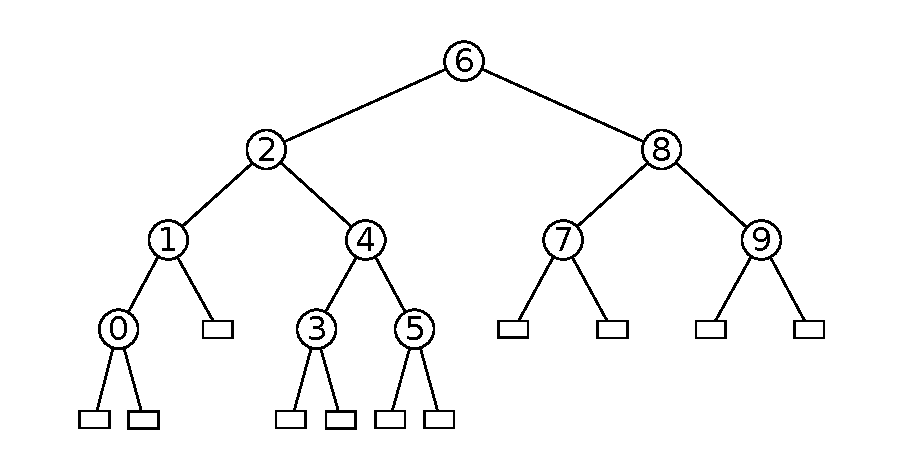
\includegraphics[width=\textwidth] {img/bin_search_tree}}
	\caption{Бинарное дерево поиска}
	\label{fig:bin_search_tree}
\end{figure}

Извлечём значения узлов в виде сортированного списка при помощи инфиксного
просмотра следующей функцией:

\begin{lstlisting}[language=OCaml]
# let rec list_of_tree = function
    Empty -> []
  | Node(lb, r, rb) -> (list_of_tree lb) @ (r :: (list_of_tree rb)) ;;
val list_of_tree : 'a arbre_bin -> 'a list = <fun>
\end{lstlisting}

Для того чтобы получить из списка бинарное дерево, определим функцию:

\begin{lstlisting}[language=OCaml]
# let rec ajout x = function
    Empty  ->  Node(Empty, x, Empty)
  | Node(fg, r, fd)  ->  if x < r then Node(ajout x fg, r, fd)
                         else Node(fg, r, ajout x fd) ;;
val ajout : 'a -> 'a arbre_bin -> 'a arbre_bin = <fun>
\end{lstlisting}

Функция трансформирующая список в бинарное дерево может быть получена
использованием функции \texttt{ajout}

\begin{lstlisting}[language=OCaml]
# let rec arbre_of_list = function
      []   ->  Empty
   | t::q  ->  ajout t (arbre_of_list q)  ;;
val arbre_of_list : 'a list -> 'a arbre_bin = <fun>
\end{lstlisting}

Тогда функция сортировки это всего--навсего композиция функций
\texttt{arbre\_of\_list} и \texttt{list\_of\_arbre}.

\begin{lstlisting}[language=OCaml]
# let tri x = list_of_arbre (arbre_of_list x) ;;
val tri : 'a list -> 'a list = <fun>
# tri [5; 8; 2; 7; 1; 0; 3; 6; 9; 4] ;;
- : int list = [0; 1; 2; 3; 4; 5; 6; 7; 8; 9]
\end{lstlisting}

\subsubsection{Общие планарные деревья}

Воспользуемся функцией определённой в модуле List (см. \ref{??}):

\begin{itemize}
	\item \texttt{List.map}: которая применяет одну функцию ко всем элементам
списка и возвращает список результатов.

	\item \texttt{List.fold\_left}: эквивалент функции \texttt{fold\_left}
определённой на стр. \ref{sec:caml_kernel:examples:lstlisting}

	\item \texttt{List.exists} применяет функцию булевого значения ко всем
элементам и если одно из применений возвращает \texttt{true}, то результат
\texttt{true}, иначе \texttt{false}. 
\end{itemize}

Общее планарное дерево --- это дерево в котором нет ограничения на число
дочерних узлов: каждому узлу ассоциируем список дочерних узлов и длина этого
списка не ограничена.

\begin{lstlisting}[language=OCaml]
# type 'a arbre = Empty
               | Node of 'a * 'a arbre list ;;
type 'a arbre = Empty | Node of 'a * 'a arbre list
\end{lstlisting}

Пустое дерево представлено значением \texttt{Empty}, лист --- это узел без
дочерних узлов формы \texttt{Node(х,[])} или \texttt{Node(x, [
Empty ; Empty; .. ])}. Таким образом достаточно просто написать функции,
манипулирующие подобными деревьями такие как принадлежность элемента дереву или
вычисление высоты дерева.

Для проверки принадлежности элемента \texttt{e} воспользуемся следующим
алгоритмом: если дерево пустое, тогда элемент \texttt{e} не принадлежит этому
дереву, в противном случае \texttt{e} принадлежит дереву только если он равен
значению корня дерева или принадлежит дочерним узлам.

\begin{lstlisting}[language=OCaml]
val belongs : 'a -> 'a arbre -> bool = <fun>
# let rec appartient e = function
    Empty -> false
  | Node(v, fs) -> (e=v) or (List.exists (appartient e) fs) ;;
val appartient : 'a -> 'a arbre -> bool = <fun>
\end{lstlisting}

Для вычисления высоты дерева, напишем следующую функцию: высота пустого дерева
равна 0, в противном случае его высота равна высоте самого большого под--дерева
плюс 1.

\begin{lstlisting}[language=OCaml]
# let rec hauteur =
  let max_list l = List.fold_left max 0 l in
   function
     Empty -> 0
   | Node (_, fs) -> 1 + (max_list (List.map hauteur fs)) ;;
val hauteur : 'a arbre -> int = <fun>
\end{lstlisting}

\subsection{Не функциональные рекурсивные значения}

Рекурсивное объявление не функциональных значений позволяет конструировать
циклические структуры данных.

Следующее объявление создаёт циклический список одного элемента.

\begin{lstlisting}[language=OCaml]
# let rec l = 1::l ;;
val l : int list =
  [1; 1; 1; 1; 1; 1; 1; 1; 1; 1; 1; 1; 1; 1; 1; 1; 1; 1; 1; 1; 1; 1; 1; 1; 1;
   1; 1; 1; 1; 1; 1; 1; 1; 1; 1; 1; 1; 1; 1; 1; 1; 1; 1; 1; 1; 1; 1; 1; 1; 1;
   1; 1; 1; 1; 1; 1; 1; 1; 1; 1; 1; 1; 1; 1; 1; 1; 1; 1; 1; 1; 1; 1; 1; 1; 1;
   1; 1; 1; 1; 1; 1; 1; 1; 1; 1; 1; 1; 1; 1; 1; 1; 1; 1; 1; 1; 1; 1; 1; 1; 1;
   1; 1; 1; 1; 1; 1; 1; 1; 1; 1; 1; 1; 1; 1; 1; 1; 1; 1; 1; 1; 1; 1; 1; 1; 1;
   1; 1; 1; 1; 1; 1; 1; 1; 1; 1; 1; 1; 1; 1; 1; 1; 1; 1; 1; 1; 1; 1; 1; 1; 1;
   1; 1; 1; 1; 1; 1; 1; 1; 1; 1; 1; 1; 1; 1; 1; 1; 1; 1; 1; 1; 1; 1; 1; 1; 1;
   1; 1; 1; 1; 1; 1; 1; 1; 1; 1; 1; 1; 1; 1; 1; 1; 1; 1; 1; 1; 1; 1; 1; 1; 1;
   1; 1; 1; 1; 1; 1; 1; 1; 1; 1; 1; 1; 1; 1; 1; 1; 1; 1; 1; 1; 1; 1; 1; 1; 1;
   1; 1; 1; 1; 1; 1; 1; 1; 1; 1; 1; 1; 1; 1; 1; 1; 1; 1; 1; 1; 1; 1; 1; 1; 1;
   1; 1; 1; 1; 1; 1; 1; 1; 1; 1; 1; 1; 1; 1; 1; 1; 1; 1; 1; 1; 1; 1; 1; 1; 1;
   1; 1; 1; 1; 1; 1; 1; 1; 1; 1; 1; 1; 1; 1; 1; 1; 1; 1; 1; 1; 1; 1; 1; 1;
   ...]
\end{lstlisting}

Применение рекурсивной функции к подобному списку приведет к переполнению
памяти.

\begin{lstlisting}[language=OCaml]
# size l ;;
Stack overflow during evaluation (looping recursion?).
\end{lstlisting}

Структурное равенство таких списков может быть проверенно лишь в случае, когда
физическое равенство верно.

\begin{lstlisting}[language=OCaml]
l=l ;;
- : bool = true
\end{lstlisting}

В случае, если мы определим такой же новый список, не стоит использовать
проверку на структурное равенство, под угрозой зацикливания программы. Таким
образом следующая инструкция не рекомендуется.

\begin{lstlisting}[language=OCaml]
let rec l2 = 1::l2 in l=l2 ;;
\end{lstlisting}

Однако, физическое равенство остаётся возможным.

\begin{lstlisting}[language=OCaml]
# let rec l2 = 1::l2 in l==l2 ;;
- : bool = false
\end{lstlisting}

Предикат \texttt{==} сравнивает непосредственно значение или разделения
структурного объекта (одним словом равенство по адресу). Мы воспользуемся этим
тестом для того чтобы при просмотре списка, не проверять уже просмотренные
под-списки. Сначала, определим функцию \texttt{memq} которая проверяет
присутствие элемента в списке при помощи физического равенства. В это же время
функция \texttt{mem} проверяет равенство структурное. Обе функции принадлежат
модулю \texttt{List}.

\begin{lstlisting}[language=OCaml]
# let rec memq a l = match l with
     [] -> false
   | b::l -> (a==b) or (memq a l) ;;
val memq : 'a -> 'a list -> bool = <fun>
\end{lstlisting}

Функция вычисляющая размер списка определена при помощи списка уже проверенных
списков и останавливается при встрече списка второй раз.

\begin{lstlisting}[language=OCaml]
# let special_size l =
   let rec size_aux previous l = match l with
       [] -> 0
     |  _::l1  -> if memq  l previous then 0
                       else 1 + (size_aux (l::previous) l1)
   in size_aux [] l ;;
val special_size : 'a list -> int = <fun>
# special_size [1;2;3;4] ;;
- : int = 4
# special_size l ;;
- : int = 1
# let rec l1 = 1::2::l2  and  l2 = 1::2::l1 in special_size l1 ;;
- : int = 4
\end{lstlisting}
